\documentclass[11pt,a4paper]{article}

% Typeface: XeLaTeX with Latin Modern Roman (fontspec default)
\usepackage{fontspec}
\usepackage{polyglossia}
\setdefaultlanguage[variant=british]{english}

% Page: the measures of the note template (A4, 11 pt, 4.5 cm side margins, header and page count)
\usepackage[a4paper,left=4.5cm,right=4.5cm,top=4.5cm,bottom=4.1cm,headheight=14pt,headsep=0.55cm,
  footskip=0.55cm]{geometry}
\linespread{0.946}
\usepackage{fancyhdr}
\usepackage{lastpage}
\pagestyle{fancy}
\fancyhf{}
\fancyhead[L]{\small\textbf{PROJECT NOTE} $|$ ASELSAN returns}
\fancyhead[R]{\small\textbf{Compiled on:} \notedate}
\fancyfoot[C]{\small\thepage\,/\,\pageref{LastPage}}
\renewcommand{\headrulewidth}{0.4pt}

\usepackage{microtype}
\usepackage{amsmath,amssymb}
\usepackage{booktabs,array,tabularx}
\usepackage{graphicx}
\usepackage{enumitem}
\setlist{noitemsep, topsep=3pt, leftmargin=*}
\usepackage{xcolor}
\definecolor{secblue}{HTML}{1F3A5F}
\definecolor{boxback}{HTML}{EEF2F6}
\definecolor{mark}{HTML}{9B2226}
\definecolor{hl}{HTML}{FFF36B}
\usepackage{titlesec}
\titleformat{\section}{\color{secblue}\bfseries\normalsize}{\thesection.}{0.4em}{}
\titlespacing*{\section}{0pt}{10pt}{4pt}
\usepackage[font=small,labelfont=bf,labelsep=period,skip=4pt]{caption}
\usepackage[bottom]{footmisc}
\usepackage{placeins}
\setlength{\parindent}{0pt}
\setlength{\parskip}{5pt}
\setlength{\textfloatsep}{10pt}
\emergencystretch=3em

\newcommand{\notedate}{\number\day\space\ifcase\month\or January\or February\or March\or April\or May\or June\or
  July\or August\or September\or October\or November\or December\fi\space\number\year}

\newcommand{\PanelDays}{1,507}
\newcommand{\ReturnDays}{1,506}
\newcommand{\FirstDay}{2020-01-03}
\newcommand{\LastDay}{2026-01-08}
\newcommand{\CarriedBrent}{49}
\newcommand{\CarriedPctBrent}{3.3}
\newcommand{\CarriedVix}{52}
\newcommand{\CarriedPctVix}{3.5}
\newcommand{\CarriedDxy}{50}
\newcommand{\CarriedPctDxy}{3.3}
\newcommand{\CarriedUsten}{52}
\newcommand{\CarriedPctUsten}{3.5}
\newcommand{\CarriedCds}{8}
\newcommand{\CarriedPctCds}{0.5}
\newcommand{\CarriedBist}{5}
\newcommand{\CarriedPctBist}{0.3}
\newcommand{\CarriedUsdtry}{3}
\newcommand{\CarriedPctUsdtry}{0.2}
\newcommand{\CdsLast}{2026-01-08}
\newcommand{\YahooLast}{2026-01-12}
\newcommand{\CumAsels}{391}
\newcommand{\CumBist}{234}
\newcommand{\SdAsels}{2.78}
\newcommand{\SdBist}{1.77}
\newcommand{\Corr}{0.66}
\newcommand{\BetaMin}{0.46}
\newcommand{\BetaMax}{1.29}
\newcommand{\BrentLastVone}{63.40}
\newcommand{\BrentLastFinal}{63.87}
\newcommand{\VixLastVone}{15.17}
\newcommand{\VixLastFinal}{15.12}
\newcommand{\Rsq}{0.448}
\newcommand{\Nobs}{1,504}
\newcommand{\BetaBist}{1.049}
\newcommand{\BetaBistSe}{0.041}
\newcommand{\UsdLoneP}{0.033}
\newcommand{\UsdLone}{0.075}
\newcommand{\CdsLoneP}{0.075}
\newcommand{\RsqSameA}{0.444}
\newcommand{\RsqLagA}{0.014}
\newcommand{\AdjRsqLagA}{0.008}
\newcommand{\RsqSameB}{0.448}
\newcommand{\RsqLagB}{0.021}
\newcommand{\AdjRsqLagB}{0.010}
\newcommand{\RsqSameC}{0.452}
\newcommand{\RsqLagC}{0.032}
\newcommand{\AdjRsqLagC}{0.014}
\newcommand{\RsqSameD}{0.462}
\newcommand{\RsqLagD}{0.051}
\newcommand{\AdjRsqLagD}{0.022}
\newcommand{\UsdJointP}{0.034}
\newcommand{\UsdJointLagP}{0.0039}
\newcommand{\VixJointP}{0.138}
\newcommand{\VixSumP}{0.030}
\newcommand{\CdsJointP}{0.308}
\newcommand{\CdsSumP}{0.508}
\newcommand{\BrentJointP}{0.094}
\newcommand{\BrentSumP}{0.015}
\newcommand{\MinOtherLagP}{0.13}
\newcommand{\EffVix}{0.25}
\newcommand{\EffLoVix}{0.03}
\newcommand{\EffHiVix}{0.48}
\newcommand{\SdVix}{2.23}
\newcommand{\EffCds}{$-$0.06}
\newcommand{\EffLoCds}{$-$0.23}
\newcommand{\EffHiCds}{0.12}
\newcommand{\SdCds}{14.26}
\newcommand{\EffBrent}{0.23}
\newcommand{\EffLoBrent}{0.04}
\newcommand{\EffHiBrent}{0.41}
\newcommand{\SdBrent}{2.69}
\newcommand{\EffUsd}{0.14}
\newcommand{\EffLoUsd}{$-$0.04}
\newcommand{\EffHiUsd}{0.32}
\newcommand{\SdUsd}{1.10}
\newcommand{\SdUsten}{0.061}
\newcommand{\RobBetaMin}{1.040}
\newcommand{\RobBetaMax}{1.053}
\newcommand{\RobCumCdsPmin}{0.067}
\newcommand{\RobCumCdsPmax}{0.920}
\newcommand{\RobCdsLevelPmin}{0.437}
\newcommand{\RobCdsLevelPmax}{0.560}
\newcommand{\RobCumCdsLevelPmax}{0.041}
\newcommand{\RobCumCdsLevelPmin}{0.009}
\newcommand{\TestFirst}{2025-01-02}
\newcommand{\TestLast}{2026-01-08}
\newcommand{\TestDays}{256}
\newcommand{\TrainDays}{1,248}
\newcommand{\TestSd}{2.69}
\newcommand{\TestMean}{0.50}
\newcommand{\PmMin}{0.21}
\newcommand{\PmMax}{0.26}
\newcommand{\UpShare}{55.3}
\newcommand{\NonzeroDays}{255}
\newcommand{\RmseArx}{2.757}
\newcommand{\RtwoArx}{$-$0.044}
\newcommand{\DaArx}{51.4}
\newcommand{\DmPArx}{0.0264}
\newcommand{\PtPArx}{0.6428}
\newcommand{\RmseAr}{2.703}
\newcommand{\RtwoAr}{$-$0.004}
\newcommand{\DaAr}{55.3}
\newcommand{\DmPAr}{0.6890}
\newcommand{\PtPAr}{0.3003}
\newcommand{\RmseLasso}{2.704}
\newcommand{\RtwoLasso}{$-$0.004}
\newcommand{\DaLasso}{55.3}
\newcommand{\DmPLasso}{0.2247}
\newcommand{\PtPLasso}{0.4398}
\newcommand{\RmseRidge}{2.705}
\newcommand{\RtwoRidge}{$-$0.005}
\newcommand{\DaRidge}{55.3}
\newcommand{\DmPRidge}{0.4154}
\newcommand{\PtPRidge}{0.3653}
\newcommand{\RmseRf}{2.715}
\newcommand{\RtwoRf}{$-$0.013}
\newcommand{\DaRf}{55.7}
\newcommand{\DmPRf}{0.4535}
\newcommand{\PtPRf}{0.2144}
\newcommand{\RmseXgb}{2.962}
\newcommand{\RtwoXgb}{$-$0.205}
\newcommand{\DaXgb}{49.4}
\newcommand{\DmPXgb}{0.0010}
\newcommand{\PtPXgb}{0.6705}
\newcommand{\RmseZero}{2.730}
\newcommand{\RtwoZero}{$-$0.024}
\newcommand{\DaZero}{--}
\newcommand{\DmPZero}{0.0299}
\newcommand{\RmseRw}{3.833}
\newcommand{\RtwoRw}{$-$1.019}
\newcommand{\DaRw}{47.6}
\newcommand{\DmPRw}{$<$0.0001}
\newcommand{\PtPRw}{0.8278}
\newcommand{\RmsePm}{2.698}
\newcommand{\RtwoPm}{0.000}
\newcommand{\DaPm}{55.3}
\newcommand{\RmseSame}{2.482}
\newcommand{\RtwoSame}{0.154}
\newcommand{\DaSame}{65.1}
\newcommand{\DmPSame}{0.0854}
\newcommand{\PtPSame}{$<$0.0001}
\newcommand{\RmseBist}{2.467}
\newcommand{\RtwoBist}{0.164}
\newcommand{\DaBist}{64.7}
\newcommand{\DmPBist}{0.0745}
\newcommand{\PtPBist}{$<$0.0001}
\newcommand{\CwPArx}{0.898}
\newcommand{\CwPAr}{0.511}
\newcommand{\DmArxArP}{0.032}
\newcommand{\CwArxArP}{0.935}
\newcommand{\LagRtwoA}{$-$0.024}
\newcommand{\LagCwPA}{0.779}
\newcommand{\LagRtwoB}{$-$0.044}
\newcommand{\LagCwPB}{0.898}
\newcommand{\LagRtwoC}{$-$0.063}
\newcommand{\LagCwPC}{0.909}
\newcommand{\LagRtwoD}{$-$0.076}
\newcommand{\LagCwPD}{0.863}
\newcommand{\RmseVoneArx}{2.49}
\newcommand{\DaVoneArx}{64.9}
\newcommand{\DmVoneP}{0.042}
\newcommand{\XgbDiff}{0.07}
\newcommand{\PtMin}{0.21}
\newcommand{\PosMin}{91}


\begin{document}


\vspace*{14pt}
\begin{tabular}{@{}p{2.35cm}@{}p{\dimexpr\textwidth-2.35cm}@{}}
\textbf{TITLE:} & \textbf{\large Return Dynamics of ASELSAN under Global and Sovereign Risk Factors: co-movement and one-day-ahead forecasts}\\[3pt]
\textbf{SUBJECT:} & Aim, method and results of the analyses in version 2 of the repository\newline
\texttt{Return-Dynamics-of-ASELSAN-under-}\newline\texttt{Global-and-Sovereign-Risk-Factors}\\[3pt]
\textbf{AUTHOR:} & Muhammed İkbal Yılmaz (myucanlar@gmail.com)
\end{tabular}

\vspace{8pt}
\vspace{12pt}

\section{Aim and scope}

Version 1 of this project studies the daily return of ASELSAN (ticker ASELS, Borsa Istanbul) with an ARX model: its own past
returns and eight factors (BIST100, USD/TRY, Bitcoin, Brent oil, VIX, the dollar index DXY, the US 10-year yield and Turkey's
5-year sovereign CDS spread), each with lags $0, 1, 2$, estimated by OLS with Newey--West standard errors. It then compares the
ARX model with simple benchmarks and four machine-learning models over 2025 and early 2026, and concludes that ASELSAN's return
has ``modest but robust'' out-of-sample predictability. Version 2 keeps the variables, the transformations, the lag orders, the
HAC lag, the sample split and the model hyperparameters of version 1, and separates two questions that version 1 treated as one:

\begin{enumerate}
  \item \textbf{How does ASELSAN move with the factors on the same day?} This is what an ARX model with lag-0 factors measures.
  Analysis 2.
  \item \textbf{Can ASELSAN's return be forecast one day ahead?} A forecast for day $t$ may only use what is known at the close of
  day $t-1$. Analysis 3.
\end{enumerate}

Analysis 1 freezes the data, describes how series traded on different calendars are aligned, and reproduces version 1.

\section{Data and notation}

\textbf{Series.} Daily closes from Yahoo Finance for ASELS.IS, XU100.IS (BIST100), TRY=X (USD/TRY), BTC-USD, BZ=F (Brent),
\^{}VIX, DX-Y.NYB (DXY) and \^{}TNX (US 10-year yield, in per cent), downloaded once for the window of version 1 (2020-01-01
to \YahooLast) and stored in \texttt{data/yahoo\_close.csv}; and the Turkey 5-year sovereign CDS spread in basis points, the file
of version 1, which ends on \CdsLast. The source of the CDS file was not recorded in version 1; it is most likely Investing.com.

\textbf{Alignment.} Let $\mathcal T$ be the set of ASELSAN trading days and $\mathcal T_s$ the dates on which series $s$ has a
close $P^{s}_u$. On day $t \in \mathcal T$ series $s$ enters with its latest close on or before $t$:
\begin{equation}
  X^{s}_t = P^{s}_{\tau_s(t)}, \qquad \tau_s(t) = \max\{u \in \mathcal T_s : u \le t\}.
\end{equation}
Nothing is filled backwards, and the panel ends on the last ASELSAN day on which every series has its own data, \LastDay; it has
\PanelDays{} days. The age $t - \tau_s(t)$ is positive when the market of $s$ was closed on $t$ (Table 1 of
\texttt{figures/}): on \CarriedVix{} days (\CarriedPctVix\%) for VIX, \CarriedBrent{} for Brent, \CarriedDxy{} for DXY,
\CarriedUsten{} for the US yield, \CarriedCds{} for CDS, \CarriedBist{} for BIST100 and \CarriedUsdtry{} for USD/TRY.

\textbf{Transformations (as in version 1).} For the price-like series $s \in \{\mathrm{ASELS}, \mathrm{BIST100},
\mathrm{USDTRY}, \mathrm{BTC}, \mathrm{BRENT}\}$ the return in per cent is $r^{s}_t = 100\,(\ln X^{s}_t - \ln X^{s}_{t'})$,
and for $s \in \{\mathrm{VIX}, \mathrm{DXY}, \mathrm{US10Y}, \mathrm{CDS}\}$ the change is $\Delta X^{s}_t = X^{s}_t -
X^{s}_{t'}$, where $t'$ is the previous ASELSAN day. Write $y_t = r^{\mathrm{ASELS}}_t$ and $Z_t = (Z_{1,t}, \dots,
Z_{8,t})'$ for the eight transformed factors. The returns run from \FirstDay{} to \LastDay{} (\ReturnDays{} days).

\textbf{Timing.} Borsa Istanbul closes before the US markets, Brent futures and the daily Bitcoin bar do. A factor value dated
$t$ is therefore known after ASELSAN's close of day $t$, sometimes several hours after it.

\section{Models and tests}

\textbf{ARX model.} For lag orders $p$ and $q$ and a first factor lag $j_0$,
\begin{equation}
  y_t = \alpha + \sum_{i=1}^{p} \phi_i\, y_{t-i} + \sum_{k=1}^{8} \sum_{j=j_0}^{q} \beta_{k,j}\, Z_{k,t-j} + \varepsilon_t
      = x_t'\theta + \varepsilon_t .
  \label{eq:arx}
\end{equation}
$j_0 = 0$ is the model of version 1: it contains $Z_t$, which is not known before day $t$ ends, so it describes
\emph{co-movement}. $j_0 = 1$ is the \emph{forecasting} model: every regressor is known at the close of day $t-1$. Version 1 uses
$p = q = 2$, and so does version 2 unless stated otherwise.

\textbf{Estimation and standard errors.} $\hat\theta = (X'X)^{-1}X'y$, with the Newey--West (1987) covariance with Bartlett
weights and $L = 5$ lags, as in version 1:
\begin{equation}
\begin{aligned}
  \hat V &= (X'X)^{-1}\, \hat S\, (X'X)^{-1},\\
  \hat S &= \sum_t \hat u_t^2 x_t x_t' + \sum_{\ell=1}^{L} \Bigl(1 - \frac{\ell}{L+1}\Bigr)
           \sum_{t} \hat u_t \hat u_{t-\ell}\, \bigl(x_t x_{t-\ell}' + x_{t-\ell} x_t'\bigr).
\end{aligned}
\end{equation}

\textbf{Channel tests.} Version 1 states, for each factor $k$, the hypothesis $H_0: \beta_{k,j} = 0$ for all $j$, but tests
single coefficients and, for VIX and CDS, the sum of their coefficients. Version 2 tests it jointly. With $R$ the matrix that selects the $r$ coefficients of factor $k$,
\begin{equation}
  W = (R\hat\theta)'\,(R\hat V R')^{-1}\,(R\hat\theta) \;\xrightarrow{d}\; \chi^2_r \quad \text{under } H_0 .
\end{equation}
The cumulative effect $s_k = \sum_j \beta_{k,j}$ (the response of $y_t$ to a lasting unit change of $Z_k$) is tested with the
same formula and $R = (0, \dots, 1, \dots, 1, \dots, 0)$, $r = 1$. To compare factors measured in different units, $s_k$ is also
reported per standard deviation of $Z_k$: $\hat s_k \hat\sigma_{Z_k}$, with the interval
$(\hat s_k \pm 1.96\,\sqrt{R\hat V R'})\,\hat\sigma_{Z_k}$.

\textbf{Recursive forecasts.} The test sample is $\mathcal T_{\mathrm{test}}$ = \TestFirst{} to \TestLast{}
(\TestDays{} days). For every $t \in \mathcal T_{\mathrm{test}}$ every model is fitted on all rows dated before $t$ (expanding
window, refitted every day) and applied to $x_t$. The models are: zero, $\hat y_t = 0$; the prevailing mean,
$\bar y_t = \frac{1}{n_t}\sum_{u<t} y_u$ (Welch and Goyal, 2008); the random walk, $\hat y_t = y_{t-1}$; AR($p$), the model
(\ref{eq:arx}) without factors; the ARX model; and Ridge, Lasso, random forest and XGBoost given exactly the inputs of the ARX
model. The hyperparameters of the tree models are those of version 1; the Ridge and Lasso penalties are chosen from the grid of
version 1, $10^{-4}, \dots, 10^{4}$ (50 values), by five-fold cross-validation in which each fold is validated only on data after
its training data.

\textbf{Forecast evaluation.} With $e_t = \hat y_t - y_t$:
\begin{itemize}
  \item the out-of-sample $R^2$ against the prevailing mean (Campbell and Thompson, 2008),
  $R^2_{\mathrm{OS}} = 1 - \sum_t (y_t - \hat y_t)^2 \big/ \sum_t (y_t - \bar y_t)^2$; it is positive when the model has the
  smaller squared error;
  \item the Diebold--Mariano (1995) test of equal squared-error loss with the correction of Harvey, Leybourne and Newbold (1997).
  For one-step forecasts and $d_t = e_{1,t}^2 - e_{2,t}^2$,
  \begin{equation}
    \begin{aligned}
    \mathrm{DM} &= \frac{\bar d}{\sqrt{\hat\sigma_d^2/T}}\sqrt{\frac{T-1}{T}}, \qquad
    \hat\sigma_d^2 = \frac1T\sum_t (d_t - \bar d)^2,\\
    \mathrm{DM} &\sim t_{T-1}\ \text{(two-sided)};
    \end{aligned}
  \end{equation}
  \item the Clark--West (2007) test for nested models. If the small model (forecast $\hat y_{1,t}$) is nested in the large one
  ($\hat y_{2,t}$), the large model's squared error is biased upwards under the null by the noise of its extra estimated
  coefficients. The test adjusts for this,
  \begin{equation}
    f_t = (y_t - \hat y_{1,t})^2 - \bigl[(y_t - \hat y_{2,t})^2 - (\hat y_{1,t} - \hat y_{2,t})^2\bigr], \qquad
    \mathrm{CW} = \frac{\bar f}{s_f/\sqrt T},
  \end{equation}
  and rejects equal accuracy in favour of the large model when CW exceeds the one-sided normal critical value;
  \item directional accuracy $\hat P$, the share of days with $\operatorname{sign}\hat y_t = \operatorname{sign} y_t$ (days with
  $y_t = 0$ or $\hat y_t = 0$ excluded), and the Pesaran--Timmermann (1992) test of independence between predicted and realized
  signs. With $\hat P_y$, $\hat P_f$ the shares of positive returns and positive forecasts,
  $P_* = \hat P_y \hat P_f + (1-\hat P_y)(1-\hat P_f)$ is the accuracy expected by chance, and
  \begin{equation}
    \mathrm{PT} = \frac{\hat P - P_*}{\sqrt{\widehat{\mathrm{Var}}(\hat P) - \widehat{\mathrm{Var}}(P_*)}}
    \;\sim\; N(0,1)\ \text{(one-sided)}.
  \end{equation}
  A forecast that never changes sign has no PT statistic: its accuracy is the share of days that went its way.
\end{itemize}

\section{Analysis 1: The data and version 1 reproduced (Figure~\ref{fig:data})}

\textbf{Why.} Version 1 downloaded the Yahoo series at every run, up to the day of the run, so its numbers could not be
reproduced, and its last row was taken during the trading day.

\textbf{Method.} The series are downloaded once and stored with the versions of the software used. The code of version 1 is run
unchanged on the stored data (\texttt{aselsan/legacy.py}). Its last row (12 January 2026) is compared with the final closes of
that day.

\textbf{How to read the figure.} (a) $\sum_{u \le t} r_u$ for ASELSAN and BIST100. (b) The slope of $r^{\mathrm{ASELS}}$ on
$r^{\mathrm{BIST}}$ in the previous 120 days, as in version 1.

\begin{figure}[!htb]
\centering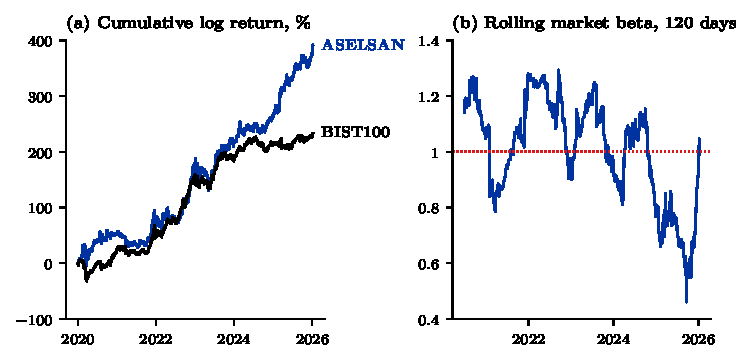
\includegraphics[width=\textwidth]{../figures/fig1_data.pdf}
\caption{ASELSAN and BIST100, \FirstDay{} to \LastDay.}\label{fig:data}
\end{figure}

\begin{table}[!htb]
\centering\small
\caption{Version 1: printed results and the same code run on the frozen data.}\label{tab:rep}
\begin{tabularx}{\textwidth}{@{}X>{\raggedleft\arraybackslash}p{1.9cm}>{\raggedleft\arraybackslash}p{2.5cm}@{}}
\toprule
Quantity & Printed by version 1 & Version 1's code, frozen data \\
\midrule
Observations in the ARX model & 1,507 & 1,506 \\
$R^2$ of the ARX model & 0.4477 & 0.4478 \\
Coefficient of $r^{\mathrm{BIST}}_t$ & 1.0494 & 1.0495 \\
$p$-value of $r^{\mathrm{USD}}_{t-1}$ & 0.0334 & 0.0343 \\
RMSE, ARX & 2.4903 & 2.4945 \\
RMSE, zero forecast & 2.7440 & 2.7493 \\
RMSE, AR & 2.7099 & 2.7158 \\
RMSE, Lasso & 2.4746 & 2.4794 \\
RMSE, random forest & 2.4982 & 2.5035 \\
RMSE, XGBoost & 2.6994 & 2.6252 \\
Directional accuracy of ARX (\%) & 64.86 & 65.12 \\
Test days & 259 & 258 \\
DM $p$-value, ARX against zero & 0.0424 & 0.0419 \\
\bottomrule

\end{tabularx}
\end{table}

\textbf{Finding.} Version 1's code on the frozen data gives its printed results to within 0.01 for $R^2$, the market
coefficient and the RMSEs of all models except XGBoost (Table~\ref{tab:rep}); the frozen data have one ASELSAN day fewer than the
data of version 1. XGBoost differs most, by \XgbDiff. In the last row of version 1 Brent was \BrentLastVone{} against a final close of
\BrentLastFinal, and VIX \VixLastVone{} against \VixLastFinal; the CDS file had no value for that day, so version 1 carried the
value of 8 January forward, which made the last two CDS changes zero. Over the panel ASELSAN's cumulative log return was \CumAsels\%
against \CumBist\% for BIST100; its daily standard deviation was \SdAsels{} per cent against \SdBist, the correlation \Corr. The
120-day market beta moved between \BetaMin{} and \BetaMax.

\textbf{Interpretation.} The results of version 1 are reproducible to the stated precision. Version 2 uses the frozen data and
ends the panel on the last CDS date, so that no series is carried past its own end.

\section{Analysis 2: Co-movement on the same day (Figure~\ref{fig:comove}, Table~\ref{tab:channels})}

\textbf{Why.} The ARX model of version 1 ($j_0 = 0$) describes how ASELSAN moves with the factors on the same day. Version 1 read
it channel by channel from single coefficients.

\textbf{Method.} Model (\ref{eq:arx}) with $j_0 = 0$, $p = q = 2$, HAC with 5 lags; joint Wald test and cumulative effect for
each channel; the same model with $j_0 = 1$; in-sample $R^2$ of both for $p = q \in \{1, 2, 3, 5\}$; and the robustness grid of
version 1 (VIX and CDS in levels or in changes, $p = q \in \{1, 3, 5\}$).

\textbf{How to read.} Table~\ref{tab:channels}: $p$-values of the joint test of all coefficients of a channel and of its
cumulative effect; the effect of a one-standard-deviation change in percentage points of ASELSAN return, with its 95\% interval;
and the joint test when the lag-0 term is removed. Figure~\ref{fig:comove}(a): $R^2$ with and without the same-day factors. (b):
the effects of the table.

\begin{table}[!htb]
\centering\small
\caption{Channels in the ARX model, $p = q = 2$, $N = \Nobs$, Newey--West with 5 lags. Effects in percentage points of the
ASELSAN return per standard deviation of the factor, lags 0--2.}\label{tab:channels}
\footnotesize\setlength{\tabcolsep}{4pt}
\begin{tabular}{@{}>{\raggedright\arraybackslash}p{2.25cm}rrcr@{}}
\toprule
 & \multicolumn{3}{c}{Same-day model ($j_0 = 0$)} & Lagged ($j_0 = 1$) \\
\cmidrule(lr){2-4}\cmidrule(l){5-5}
Channel & joint $p$ & cumulative $p$ & effect per s.d. [95\% CI] & joint $p$ \\
\midrule
market (BIST100) & $<$0.0001 & $<$0.0001 & -- & 0.6293 \\
exchange rate (USD/TRY) & 0.0335 & 0.1382 & 0.14 [$-$0.04, 0.32] & 0.0039 \\
global risk (VIX) & 0.1376 & 0.0296 & 0.25 [0.03, 0.48] & 0.6661 \\
sovereign risk (CDS) & 0.3079 & 0.5082 & $-$0.06 [$-$0.23, 0.12] & 0.3294 \\
dollar (DXY) & 0.4630 & 0.4362 & $-$0.09 [$-$0.31, 0.14] & 0.1591 \\
US 10-year yield & 0.4279 & 0.1574 & $-$0.15 [$-$0.36, 0.06] & 0.6184 \\
Bitcoin & 0.7087 & 0.9852 & 0.00 [$-$0.18, 0.18] & 0.8296 \\
Brent oil & 0.0937 & 0.0153 & 0.23 [0.04, 0.41] & 0.1328 \\
\bottomrule

\end{tabular}
\end{table}

\begin{figure}[!htb]
\centering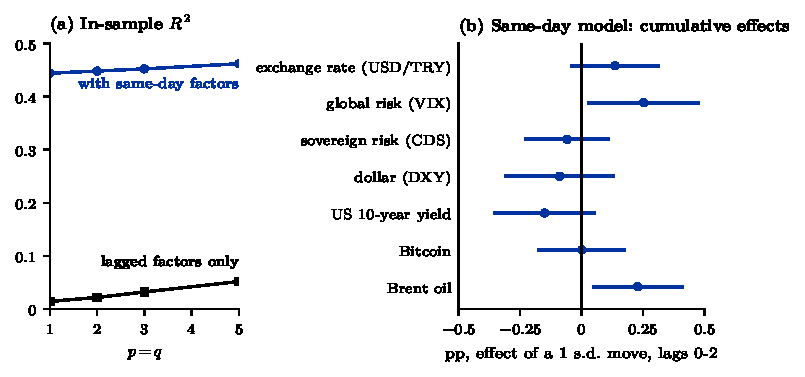
\includegraphics[width=\textwidth]{../figures/fig2_comovement.pdf}
\caption{(a) In-sample $R^2$ of model (\ref{eq:arx}) with $j_0 = 0$ and $j_0 = 1$. (b) Cumulative effect of a
one-standard-deviation change of each factor (lags 0--2) with 95\% HAC interval.}\label{fig:comove}
\end{figure}

\textbf{Finding.} The model of version 1 is reproduced: $R^2 = \Rsq$, market coefficient \BetaBist{} (s.e.\ \BetaBistSe). Almost
all of the fit comes from the same day: without the lag-0 terms $R^2$ falls from \RsqSameB{} to \RsqLagB{} (adjusted
\AdjRsqLagB), and with five lags it is \RsqLagD{} (Figure~\ref{fig:comove}a). Tested jointly, the exchange-rate channel
is significant on the same day ($p = \UsdJointP$) and is the only lagged channel that is ($p = \UsdJointLagP$); the other lagged
channels have $p \ge \MinOtherLagP$. VIX and Brent are not significant as channels ($p = \VixJointP$ and \BrentJointP), but their
cumulative effects are ($p = \VixSumP$ and \BrentSumP): a one-standard-deviation rise of VIX (\SdVix{} points) goes with
\EffVix{} [\EffLoVix, \EffHiVix] percentage points higher ASELSAN return over three days, and of Brent (\SdBrent\%) with \EffBrent{}
[\EffLoBrent, \EffHiBrent]. The CDS channel is not significant in any form in the baseline: joint $p = \CdsJointP$, cumulative $p =
\CdsSumP$, effect \EffCds{} [\EffLoCds, \EffHiCds]. In the robustness grid the market coefficient stays between \RobBetaMin{} and
\RobBetaMax; the cumulative effect of CDS changes has $p$ between \RobCumCdsPmin{} and \RobCumCdsPmax; the sum of the CDS level
coefficients has $p$ between \RobCumCdsLevelPmin{} and \RobCumCdsLevelPmax.

\textbf{Interpretation.} ASELSAN is a market stock with a beta near one; beyond the market, its same-day return moves with the
exchange rate, and its three-day cumulative response is positive to VIX and to oil. A joint test asks whether any coefficient of
the channel differs from zero; the cumulative test asks about one direction, their sum, and has more power when the coefficients
share a sign. With a lower bound of \EffLoVix{}, the VIX effect is imprecisely estimated. The negative CDS result that version 1 reported does not survive in changes. In levels the
sum of the coefficients is the coefficient on a very persistent regressor, for which the normal approximation behind these
$p$-values is not reliable, so that result is not taken as evidence. None of this is a forecast: the same-day values are not
known in advance, and the US and oil closes of day $t$ are set after Borsa Istanbul closes.

\section{Analysis 3: One-day-ahead forecasts (Figure~\ref{fig:fc}, Table~\ref{tab:fc})}

\textbf{Why.} Version 1's ``out-of-sample forecasts'' for day $t$ used the factors of day $t$, and its machine-learning models were
given every column of its data table, including the same-day prices and returns of the factors and the closing price of ASELSAN
on day $t$. They measure how well the return can be explained once the day is over. Version 1 reported RMSE \RmseVoneArx{} and
directional accuracy \DaVoneArx\% for its ARX model, and a Diebold--Mariano $p = \DmVoneP$ against the zero forecast.

\textbf{Method.} Recursive forecasts for the \TestDays{} test days (first training sample: \TrainDays{} days). In the forecasting
design ($j_0 = 1$, $p = q = 2$) every input is known at the close of day $t-1$. For comparison, the same-day design of version 1
and a model with the same-day BIST100 return alone. The benchmark is the prevailing mean, the standard benchmark in this
literature (Welch and Goyal, 2008; Rapach and Zhou, 2013); Clark--West is used for the nested linear models.

\textbf{How to read.} Table~\ref{tab:fc}: RMSE in percentage points; $R^2_{\mathrm{OS}}$ against the prevailing mean;
directional accuracy (\%) and the PT $p$-value; DM $p$-value against the prevailing mean; CW $p$-value against the prevailing mean.
Figure~\ref{fig:fc}: $\sum_{u \le t} [(y_u - \bar y_u)^2 - (y_u - \hat y_u)^2]$; a rising line means the model is gaining on the
prevailing mean.

\begin{table}[!htb]
\centering\small
\caption{One-day-ahead forecasts, \TestFirst{} to \TestLast{} (\TestDays{} days), recursive and refitted daily.}\label{tab:fc}
\footnotesize\setlength{\tabcolsep}{4pt}
\begin{tabular}{@{}lrrrrrr@{}}
\toprule
Model & RMSE & $R^2_{\mathrm{OS}}$ & Dir.\ acc. & PT $p$ & DM $p$ & CW $p$ \\
\midrule
Zero & 2.730 & $-$0.024 & -- & -- & 0.0299 & -- \\
Prevailing mean & 2.698 & 0.000 & 55.3 & -- & -- & -- \\
Random walk & 3.833 & $-$1.019 & 47.6 & 0.8278 & $<$0.0001 & -- \\
AR & 2.703 & $-$0.004 & 55.3 & 0.3003 & 0.6890 & 0.5108 \\
ARX & 2.757 & $-$0.044 & 51.4 & 0.6428 & 0.0264 & 0.8979 \\
Ridge & 2.705 & $-$0.005 & 55.3 & 0.3653 & 0.4154 & -- \\
Lasso & 2.704 & $-$0.004 & 55.3 & 0.4398 & 0.2247 & -- \\
Random forest & 2.715 & $-$0.013 & 55.7 & 0.2144 & 0.4535 & -- \\
XGBoost & 2.962 & $-$0.205 & 49.4 & 0.6705 & 0.0010 & -- \\
\midrule
\multicolumn{7}{l}{\emph{Same-day factors (design of version 1, not a forecast)}} \\
ARX, same-day factors & 2.482 & 0.154 & 65.1 & $<$0.0001 & 0.0854 & -- \\
BIST100 same day only & 2.467 & 0.164 & 64.7 & $<$0.0001 & 0.0745 & -- \\
\bottomrule

\end{tabular}
\end{table}

\begin{figure}[!htb]
\centering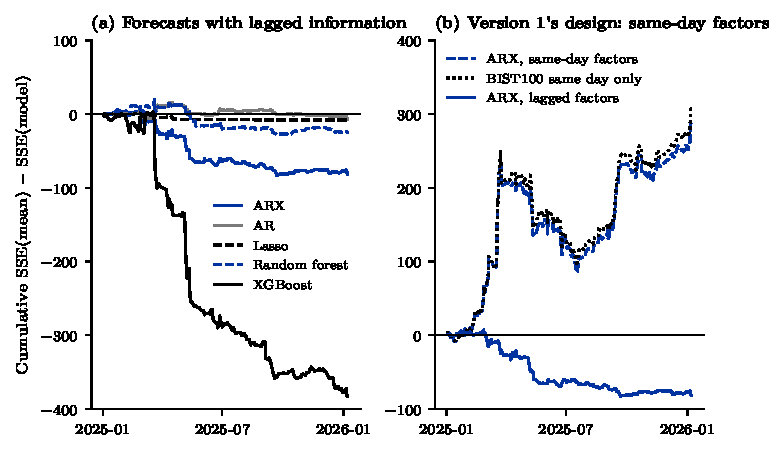
\includegraphics[width=\textwidth]{../figures/fig3_forecasts.pdf}
\caption{Cumulative difference of squared errors, prevailing mean minus model. (a) Forecasts with information up to $t-1$.
(b) The same-day design of version 1 against the lagged ARX model.}\label{fig:fc}
\end{figure}

\textbf{Finding.} With information up to day $t-1$ no model beats the prevailing mean. The ARX model has $R^2_{\mathrm{OS}}$ =
\RtwoArx{} and is significantly worse than the mean (DM $p = \DmPArx$) and than the AR model (DM $p = \DmArxArP$); Clark--West
finds no gain from the factors ($p = \CwPArx$ against the mean, \CwArxArP{} against AR). Ridge, Lasso and AR are close to the mean
($R^2_{\mathrm{OS}}$ \RtwoRidge, \RtwoLasso, \RtwoAr): they forecast a rise on at least \PosMin\% of the days, and their directional accuracy,
\DaLasso\%, equals the share of rising days among the \NonzeroDays{} non-zero returns, \UpShare\%. The random forest has
\RtwoRf; XGBoost, \RtwoXgb, is significantly worse than the mean (DM $p = \DmPXgb$). No directional accuracy differs from chance
(PT $p \ge \PtMin$). More lags make the ARX model worse: $R^2_{\mathrm{OS}}$ is \LagRtwoA, \LagRtwoB, \LagRtwoC{} and \LagRtwoD{}
for $p = q = 1, 2, 3, 5$. With the same-day factors of version 1 the picture reverses: $R^2_{\mathrm{OS}} = \RtwoSame$ and
directional accuracy \DaSame\% (PT $p$ \PtPSame), close to version 1's results. The same-day BIST100 return alone does as well
($R^2_{\mathrm{OS}} = \RtwoBist$, \DaBist\%).

\textbf{Interpretation.} The accuracy reported by version 1 comes from the same-day market return, which is not known when the
forecast would have to be made. Once the information set is restricted to day $t-1$, the factors carry no forecasting power for
ASELSAN's daily return in the test period; the models whose forecasts stay close to the mean (AR, Ridge,
Lasso) lose least, and XGBoost loses most. This agrees with the general
finding that daily stock returns are hard to forecast beyond their historical mean (Welch and Goyal, 2008; Rapach and Zhou, 2013).
Two points limit the strength of this conclusion: the test sample is one year, and returns are heavy-tailed, so a few days carry a
large share of the squared errors; Figure~\ref{fig:fc}(b) shows the jumps of single days. Even the same-day $R^2_{\mathrm{OS}}$ of
\RtwoSame{} has a DM $p$-value of only \DmPSame.

\section{Conclusions and limitations}

\begin{itemize}
  \item ASELSAN's daily return moves with the market (beta \BetaBist) and, beyond it, with the exchange rate; its cumulative
  same-day response to VIX and Brent is positive; sovereign CDS changes show no significant relation in the baseline.
  \item These are same-day relations. With information up to the previous close, neither the ARX model nor Ridge, Lasso, random
  forest or XGBoost forecasts the next day's return better than the prevailing mean in 2025--2026.
  \item Limitations: one test year; a single stock; the factor closes of the US and oil markets are set after Borsa Istanbul
  closes, so even the same-day relations mix information from different hours; the CDS series comes from a file whose source was not
  recorded; Yahoo's adjusted prices can be revised, which is why the downloaded data are stored with the repository.
\end{itemize}

\section*{References}
{\small
\setlength{\parskip}{2pt}
\hangindent=1.27cm\hangafter=1 Campbell, J. Y., \& Thompson, S. B. (2008). Predicting excess stock returns out of sample: can anything beat the historical average?
\textit{Review of Financial Studies}, 21(4), 1509--1531.\par
\hangindent=1.27cm\hangafter=1 Clark, T. E., \& West, K. D. (2007). Approximately normal tests for equal predictive accuracy in nested models. \textit{Journal of
Econometrics}, 138(1), 291--311.\par
\hangindent=1.27cm\hangafter=1 Diebold, F. X., \& Mariano, R. S. (1995). Comparing predictive accuracy. \textit{Journal of Business \& Economic Statistics}, 13(3),
253--263.\par
\hangindent=1.27cm\hangafter=1 Harvey, D., Leybourne, S., \& Newbold, P. (1997). Testing the equality of prediction mean squared errors. \textit{International
Journal of Forecasting}, 13(2), 281--291.\par
\hangindent=1.27cm\hangafter=1 Newey, W. K., \& West, K. D. (1987). A simple, positive semi-definite, heteroskedasticity and autocorrelation consistent covariance
matrix. \textit{Econometrica}, 55(3), 703--708.\par
\hangindent=1.27cm\hangafter=1 Pesaran, M. H., \& Timmermann, A. (1992). A simple nonparametric test of predictive performance. \textit{Journal of Business \&
Economic Statistics}, 10(4), 461--465.\par
\hangindent=1.27cm\hangafter=1 Rapach, D. E., \& Zhou, G. (2013). Forecasting stock returns. In G. Elliott \& A. Timmermann (Eds.), \textit{Handbook of Economic
Forecasting} (Vol. 2A, pp. 328--383). Elsevier.\par
\hangindent=1.27cm\hangafter=1 Welch, I., \& Goyal, A. (2008). A comprehensive look at the empirical performance of equity premium prediction. \textit{Review of
Financial Studies}, 21(4), 1455--1508.\par

\smallskip
All numbers are generated from
\texttt{figures/*.csv} by \texttt{make\_paper.py}.
}

\end{document}
